\documentclass[]{article}
\usepackage{lmodern}
\usepackage{amssymb,amsmath}
\usepackage{ifxetex,ifluatex}
\usepackage{hyperref}
\usepackage{fixltx2e} % provides \textsubscript
\usepackage{cleveref}
\usepackage{enumitem}
\usepackage{graphicx}
\usepackage{tikz}

\ifnum 0\ifxetex 1\fi\ifluatex 1\fi=0 % if pdftex
  \usepackage[T1]{fontenc}
  \usepackage[utf8]{inputenc}
\else % if luatex or xelatex
  \ifxetex
    \usepackage{mathspec}
  \else
    \usepackage{fontspec}
  \fi
  \defaultfontfeatures{Ligatures=TeX,Scale=MatchLowercase}
\fi
% use upquote if available, for straight quotes in verbatim environments
\IfFileExists{upquote.sty}{\usepackage{upquote}}{}
% use microtype if available
\IfFileExists{microtype.sty}{%
\usepackage[]{microtype}
\UseMicrotypeSet[protrusion]{basicmath} % disable protrusion for tt fonts
}{}
\PassOptionsToPackage{hyphens}{url} % url is loaded by hyperref
\usepackage[unicode=true]{hyperref}
\hypersetup{
            pdfborder={0 0 0},
            breaklinks=true}
\urlstyle{same}  % don't use monospace font for urls
\IfFileExists{parskip.sty}{%
\usepackage{parskip}
}{% else
\setlength{\parindent}{0pt}
\setlength{\parskip}{6pt plus 2pt minus 1pt}
}
\setlength{\emergencystretch}{3em}  % prevent overfull lines
\providecommand{\tightlist}{%
  \setlength{\itemsep}{0pt}\setlength{\parskip}{0pt}}
\setcounter{secnumdepth}{0}
% Redefines (sub)paragraphs to behave more like sections
\ifx\paragraph\undefined\else
\let\oldparagraph\paragraph
\renewcommand{\paragraph}[1]{\oldparagraph{#1}\mbox{}}
\fi
\ifx\subparagraph\undefined\else
\let\oldsubparagraph\subparagraph
\renewcommand{\subparagraph}[1]{\oldsubparagraph{#1}\mbox{}}
\fi

% set default figure placement to htbp
\makeatletter
\def\fps@figure{htbp}
\makeatother

\title{CS 182: Problem Set 5}
\author{Alan Turing}
\date{\today}

\begin{document}

\maketitle

\textbf{Introduction:}  
Welcome to the last official homework for CS182!  As you are hopefully already aware, this PDF comprises the written component of the second problem set.  In addition to solving the problems found below, you will also need to complete the coding part of the assignment, found in the Github repo.  Finally, we'd like to remind you that while you are allowed a partner for the coding part of the assignment, you are \textbf{NOT} allowed a partner for this and all future written components.  All written work should be yours and yours alone.  This being said, in addition to being able to ask questions at office hours, you are allowed to discuss questions with fellow classmates, provided 1) you note the people with whom you collaborated, and 2) you \textbf{DO NOT} copy any answers.  Please write up the solutions to all problems independently.

\bigskip
\textbf{Collaborators:}

\clearpage

\textbf{Problem 1 (Coin Flipping) -- 4 Points:}
We have a bag of three biased coins a, b, and c with probabilities of coming up heads of 20\%, 60\%, and 80\%, respectively. One coin is drawn randomly from the bag (with equal likelihood of drawing each of the three coins), and then the coin is flipped three times to generate the outcomes X1, X2, and X3.

\begin{enumerate}[label=(\alph*)]
    \item (2 points) Draw the Bayesian network corresponding to this setup and define the necessary conditional probability tables.
    \item (2 points) Calculate which coin was most likely to have been drawn from the bag if the observed flips come out heads twice and tails once.
\end{enumerate}
\bigskip

\textbf{Solution 1:}
% TODO: Your solution for question 1

\clearpage

\textbf{Problem 2 (Bayes Nets) -- 6 Points:}
This problem uses this Bayesian Network of binary (0 or 1) random variables:
\begin{center}
    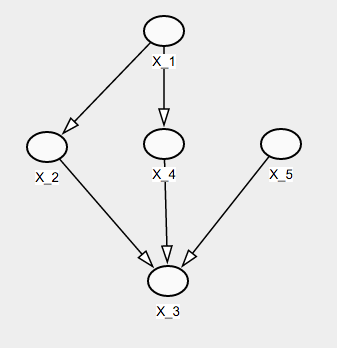
\includegraphics[width=5cm]{BN.png}
\end{center}

\begin{enumerate}[label=(\alph*)]
    \item (2 points) For a binary random variable $X$, a single value $P(X=0)$ can explain the entire distribution as $P(X=1) = 1-P(X=0)$. What's the minimum number of values needed to completely explain the joint probability distribution of the provided Bayesian Network?
    \item (2 points) Which nodes are dependent on $X_2$, meaning $P(X_i|X_2) \neq P(X_i)$? Why?
    \item (2 points) Which nodes are dependent on $X_2$ if $X_3$ is given?
\end{enumerate}
\bigskip

\textbf{Solution 2:}
% TODO: Your solution for question 2

\clearpage

\textbf{Problem 3 (HMMs) -- 7 Points:}
It's the busiest time of the semester, and you have so much work to do that your eating schedule has gone out of whack. On a given day, your state is either very hungry or you've eaten so much food that you've become very sleepy. You have an observable behavior based on your state of being either gregarious, aloof, or violently angry. Your given HMM model is:

\begin{table}[!htb]
\centering
    \begin{tabular}{|c|c|}
        \hline
         & $P(S_1)$ \\\hline
         hungry & 1 \\\hline
         sleepy & 0 \\\hline
    \end{tabular}
\end{table}
\begin{table}[!htb]
\centering
    \begin{tabular}{|c|c|}
        \hline
         & $P(S_t|S_{t-1}=hungry)$ \\\hline
         hungry & 1/4 \\\hline
         sleepy & 3/4 \\\hline
    \end{tabular}
\end{table}
\begin{table}[!htb]
\centering
    \begin{tabular}{|c|c|}
        \hline
         & $P(S_t|S_{t-1}=sleepy)$ \\\hline
         hungry & 3/4 \\\hline
         sleepy & 1/4 \\\hline
    \end{tabular}
\end{table}
\begin{table}[!htb]
\centering
    \begin{tabular}{|c|c|}
        \hline
         & $P(B_t|S_t=hungry)$ \\\hline
         gregarious & 1/4 \\\hline
         aloof & 1/4 \\\hline
         violent & 1/2 \\\hline
    \end{tabular}
\end{table}
\begin{table}[!htb]
\centering
    \begin{tabular}{|c|c|}
        \hline
         & $P(B_t|S_t=sleepy)$ \\\hline
         gregarious & 1/4 \\\hline
         aloof & 3/4 \\\hline
         violent & 0 \\\hline
    \end{tabular}
\end{table}

\begin{enumerate}[label=(\alph*)]
    \item (3 points) What is $P(S_2 = hungry | B_2 = aloof)$?
    \item (2 points) Using the utilities below, what is the expected utility of your friend talking to you if your friend hadn't observed your behavior?
    
    \begin{table}[!htb]
    \centering
        \begin{tabular}{|c|c|}
            \hline
             $S_2$ & U \\\hline
             hungry & -2 \\\hline
             sleepy & 3 \\\hline
        \end{tabular}
    \end{table}
    
    \item (2 points) Now what is the expected utility if your friend sees you're aloof?
\end{enumerate}

\bigskip

\textbf{Solution 3:}
% TODO: Your solution for question 3

\clearpage

\textbf{Problem 4 (Bayes Nets) -- 8 Points:}

Consider the Bayes net shown below, with Boolean variables $B = BrokeElectionLaw$, $I = Indicted$, $M = PoliticallyMotivatedProsecutor$, $G = FoundGuilty$, and $J = Jailed$.

\begin{center}
    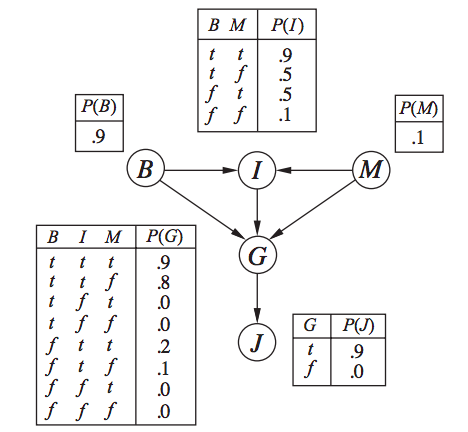
\includegraphics[width=6cm]{BN2.png}
\end{center}

\begin{enumerate}[label=(\alph*)]
    \item (3 points) Which of the following are asserted by the network structure? Briefly explain.
    
    \begin{itemize}
        \item[] (i) $P(B,I,M) = P(B)P(I)P(M)$
        \item[] (ii) $P(J | G) = P(J | G, I)$
        \item[] (iii) $P(M | G, B, I) = P(M | G, B, I, J)$
    \end{itemize}
    
    \item (2 points) Calculate the value of $P(b, i, \neg m, g, j)$.
    \item (2 points) Calculate the probability that someone goes to jail given that they broke the law, have been indicted, and face a politically motivated prosecutor.
    \item (1 point) Suppose we want to add the variable $P = PresidentialPardon$ to the network; draw the new network and briefly explain any links you add.

\end{enumerate}

\bigskip

\textbf{Solution 4:}
% TODO: Your solution for question 4

\end{document}

